\documentclass[11pt]{article}
\usepackage[margin=1.0cm, paperwidth=8.5in, paperheight=14in]{geometry}
\usepackage{tikz}
\usepackage{amsmath,amssymb}
\usepackage{xcolor}
\usetikzlibrary{calc,positioning}

\definecolor{orange1}{RGB}{230,130,20}
\definecolor{red1}{RGB}{210,40,40}
\definecolor{green1}{RGB}{50,180,80}
\definecolor{magenta1}{RGB}{200,40,160}

\pagestyle{empty}

% Hexagon drawing command - define OUTSIDE tikzpicture
% Usage: \drawhex{x}{y}{radius}{diagonal commands}
\newcommand{\drawhex}[4]{%
  \foreach \a/\n [remember=\a as \lasta (initially 330)] in {90/1,150/2,210/3,270/4,330/5,30/6}{
    \coordinate (v\n) at ([shift={(#1,#2)}]\a:#3);
  }
  \draw[thick] ([shift={(#1,#2)}]90:#3)--([shift={(#1,#2)}]150:#3)--([shift={(#1,#2)}]210:#3)--([shift={(#1,#2)}]270:#3)--([shift={(#1,#2)}]330:#3)--([shift={(#1,#2)}]30:#3)--cycle;
}

\begin{document}

\begin{tikzpicture}[remember picture, overlay]
  \node[anchor=north east, orange1, font=\large] at ([xshift=-1.5cm, yshift=-0.8cm]current page.north east)
    {$X_{2\delta} = X_{1\delta} - X_{13}$};
\end{tikzpicture}

\vspace{0.2cm}

{\large\itshape all \quad possible \quad diagrams \quad with \quad 6 \quad legs}

\smallskip
{\itshape group \quad them \quad by}

\vspace{0.3cm}

% ============================================================
% ROW 1: Three LARGE labeled hexagons
% ============================================================
\begin{center}
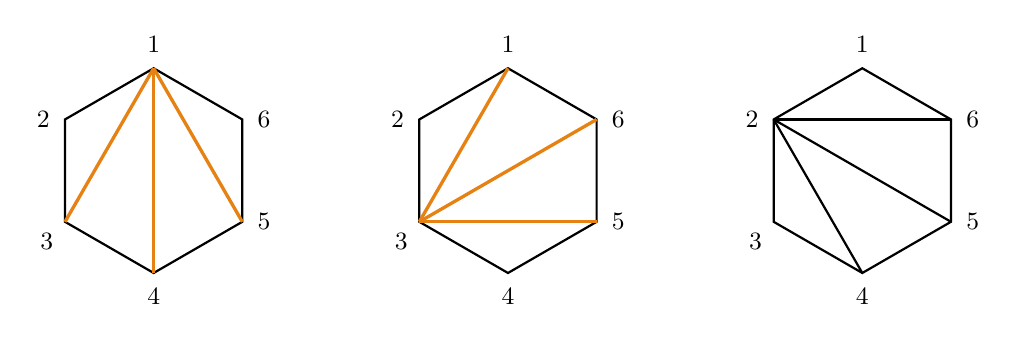
\begin{tikzpicture}[scale=1.0]

% Hex 1: fan from vertex 1 (orange)
\foreach \a/\n in {90/1,150/2,210/3,270/4,330/5,30/6}
  \coordinate (a\n) at (\a:1.3);
\draw[thick] (a1)--(a2)--(a3)--(a4)--(a5)--(a6)--cycle;
\draw[orange1, very thick] (a1)--(a3); \draw[orange1, very thick] (a1)--(a4); \draw[orange1, very thick] (a1)--(a5);
\node[above=2pt] at (a1) {\small 1}; \node[left=2pt] at (a2) {\small 2};
\node[below left=1pt] at (a3) {\small 3}; \node[below=2pt] at (a4) {\small 4};
\node[right=2pt] at (a5) {\small 5}; \node[right=2pt] at (a6) {\small 6};

% Hex 2: fan from vertex 3 (orange)
\foreach \a/\n in {90/1,150/2,210/3,270/4,330/5,30/6}
  \coordinate (b\n) at ([shift={(4.5,0)}]\a:1.3);
\draw[thick] (b1)--(b2)--(b3)--(b4)--(b5)--(b6)--cycle;
\draw[orange1, very thick] (b3)--(b1); \draw[orange1, very thick] (b3)--(b5); \draw[orange1, very thick] (b3)--(b6);
\node[above=2pt] at (b1) {\small 1}; \node[left=2pt] at (b2) {\small 2};
\node[below left=1pt] at (b3) {\small 3}; \node[below=2pt] at (b4) {\small 4};
\node[right=2pt] at (b5) {\small 5}; \node[right=2pt] at (b6) {\small 6};

% Hex 3: fan from vertex 2 (black diags only)
\foreach \a/\n in {90/1,150/2,210/3,270/4,330/5,30/6}
  \coordinate (c\n) at ([shift={(9,0)}]\a:1.3);
\draw[thick] (c1)--(c2)--(c3)--(c4)--(c5)--(c6)--cycle;
\draw[thick] (c2)--(c4); \draw[thick] (c2)--(c5); \draw[thick] (c2)--(c6);
\node[above=2pt] at (c1) {\small 1}; \node[left=2pt] at (c2) {\small 2};
\node[below left=1pt] at (c3) {\small 3}; \node[below=2pt] at (c4) {\small 4};
\node[right=2pt] at (c5) {\small 5}; \node[right=2pt] at (c6) {\small 6};

\end{tikzpicture}
\end{center}

\vspace{0.1cm}

% ============================================================
% ROWS 2-4: Smaller hexagons (unlabeled), orange triangulations
% ============================================================
\begin{center}
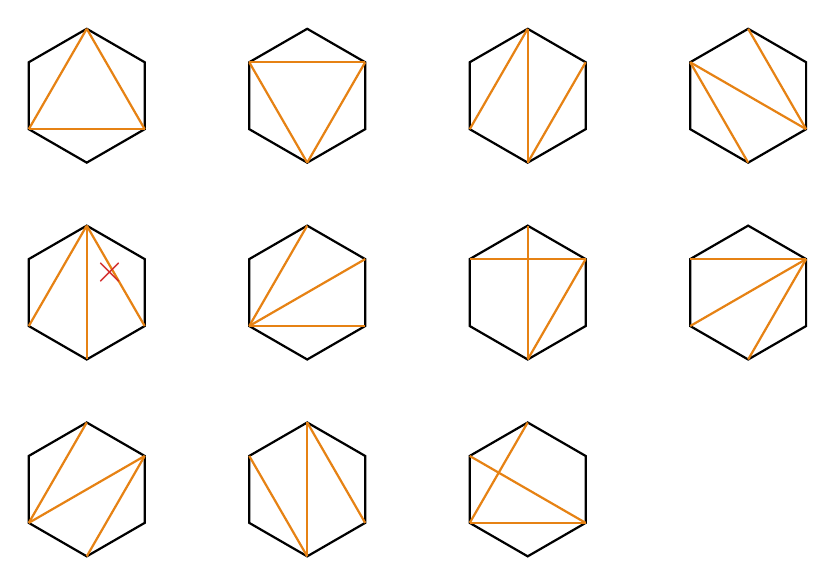
\begin{tikzpicture}[scale=1.0]

% Helper: small hex at (cx,cy) with radius 0.85
\def\R{0.85}
\def\DX{2.8}

% ----- ROW 2 (y=0): 4 hexagons -----
% H1: (1-3, 3-5, 5-1) alternate star
\foreach \a/\n in {90/1,150/2,210/3,270/4,330/5,30/6}
  \coordinate (r2a\n) at (\a:\R);
\draw[thick] (r2a1)--(r2a2)--(r2a3)--(r2a4)--(r2a5)--(r2a6)--cycle;
\draw[orange1, thick] (r2a1)--(r2a3); \draw[orange1, thick] (r2a3)--(r2a5); \draw[orange1, thick] (r2a5)--(r2a1);

% H2
\foreach \a/\n in {90/1,150/2,210/3,270/4,330/5,30/6}
  \coordinate (r2b\n) at ([shift={(\DX,0)}]\a:\R);
\draw[thick] (r2b1)--(r2b2)--(r2b3)--(r2b4)--(r2b5)--(r2b6)--cycle;
\draw[orange1, thick] (r2b2)--(r2b4); \draw[orange1, thick] (r2b4)--(r2b6); \draw[orange1, thick] (r2b6)--(r2b2);

% H3
\foreach \a/\n in {90/1,150/2,210/3,270/4,330/5,30/6}
  \coordinate (r2c\n) at ([shift={(2*\DX,0)}]\a:\R);
\draw[thick] (r2c1)--(r2c2)--(r2c3)--(r2c4)--(r2c5)--(r2c6)--cycle;
\draw[orange1, thick] (r2c1)--(r2c3); \draw[orange1, thick] (r2c1)--(r2c4); \draw[orange1, thick] (r2c4)--(r2c6);

% H4
\foreach \a/\n in {90/1,150/2,210/3,270/4,330/5,30/6}
  \coordinate (r2d\n) at ([shift={(3*\DX,0)}]\a:\R);
\draw[thick] (r2d1)--(r2d2)--(r2d3)--(r2d4)--(r2d5)--(r2d6)--cycle;
\draw[orange1, thick] (r2d2)--(r2d4); \draw[orange1, thick] (r2d2)--(r2d5); \draw[orange1, thick] (r2d5)--(r2d1);

% ----- ROW 3 (y=-2.5): 4 hexagons, first with red X -----
\def\RY{-2.5}

% H5 (red X)
\foreach \a/\n in {90/1,150/2,210/3,270/4,330/5,30/6}
  \coordinate (r3a\n) at ([shift={(0,\RY)}]\a:\R);
\draw[thick] (r3a1)--(r3a2)--(r3a3)--(r3a4)--(r3a5)--(r3a6)--cycle;
\draw[orange1, thick] (r3a1)--(r3a3); \draw[orange1, thick] (r3a1)--(r3a4); \draw[orange1, thick] (r3a1)--(r3a5);
\node[red1, font=\Large\bfseries] at ([shift={(0.3,0.25)}]0,\RY) {$\times$};

% H6
\foreach \a/\n in {90/1,150/2,210/3,270/4,330/5,30/6}
  \coordinate (r3b\n) at ([shift={(\DX,\RY)}]\a:\R);
\draw[thick] (r3b1)--(r3b2)--(r3b3)--(r3b4)--(r3b5)--(r3b6)--cycle;
\draw[orange1, thick] (r3b3)--(r3b5); \draw[orange1, thick] (r3b3)--(r3b6); \draw[orange1, thick] (r3b3)--(r3b1);

% H7
\foreach \a/\n in {90/1,150/2,210/3,270/4,330/5,30/6}
  \coordinate (r3c\n) at ([shift={(2*\DX,\RY)}]\a:\R);
\draw[thick] (r3c1)--(r3c2)--(r3c3)--(r3c4)--(r3c5)--(r3c6)--cycle;
\draw[orange1, thick] (r3c1)--(r3c4); \draw[orange1, thick] (r3c4)--(r3c6); \draw[orange1, thick] (r3c6)--(r3c2);

% H8
\foreach \a/\n in {90/1,150/2,210/3,270/4,330/5,30/6}
  \coordinate (r3d\n) at ([shift={(3*\DX,\RY)}]\a:\R);
\draw[thick] (r3d1)--(r3d2)--(r3d3)--(r3d4)--(r3d5)--(r3d6)--cycle;
\draw[orange1, thick] (r3d6)--(r3d3); \draw[orange1, thick] (r3d6)--(r3d4); \draw[orange1, thick] (r3d2)--(r3d6);

% ----- ROW 4 (y=-5.0): 3 hexagons -----
\def\RYY{-5.0}

% H9
\foreach \a/\n in {90/1,150/2,210/3,270/4,330/5,30/6}
  \coordinate (r4a\n) at ([shift={(0,\RYY)}]\a:\R);
\draw[thick] (r4a1)--(r4a2)--(r4a3)--(r4a4)--(r4a5)--(r4a6)--cycle;
\draw[orange1, thick] (r4a1)--(r4a3); \draw[orange1, thick] (r4a3)--(r4a6); \draw[orange1, thick] (r4a6)--(r4a4);

% H10
\foreach \a/\n in {90/1,150/2,210/3,270/4,330/5,30/6}
  \coordinate (r4b\n) at ([shift={(\DX,\RYY)}]\a:\R);
\draw[thick] (r4b1)--(r4b2)--(r4b3)--(r4b4)--(r4b5)--(r4b6)--cycle;
\draw[orange1, thick] (r4b2)--(r4b4); \draw[orange1, thick] (r4b4)--(r4b1); \draw[orange1, thick] (r4b1)--(r4b5);

% H11
\foreach \a/\n in {90/1,150/2,210/3,270/4,330/5,30/6}
  \coordinate (r4c\n) at ([shift={(2*\DX,\RYY)}]\a:\R);
\draw[thick] (r4c1)--(r4c2)--(r4c3)--(r4c4)--(r4c5)--(r4c6)--cycle;
\draw[orange1, thick] (r4c5)--(r4c3); \draw[orange1, thick] (r4c3)--(r4c1); \draw[orange1, thick] (r4c5)--(r4c2);

\end{tikzpicture}
\end{center}

\vspace{0.2cm}
\noindent\rule{\textwidth}{0.8pt}
\vspace{0.4cm}

% ============================================================
% TEXT SECTION
% ============================================================
{\large\itshape splitting \quad dependency \quad on \quad $z$ \quad scaling \quad of \quad propagators}

\medskip
\noindent
\fbox{\;\textit{boundary propagators}\;}: \quad the ones that scale linearly with $z$ under BCFW shift

\smallskip
\hspace{4cm} ($X_{1\delta}$ \;\;and\;\; $X_{2\delta}$)

\vspace{0.5cm}
{\large\itshape group \quad by \quad $\#$ \quad of \quad boundary \quad propagators}

\smallskip
$\Rightarrow$ \;\;\textit{group \quad them \quad by \quad scaling \quad under \quad BCFW \quad shift}

\vspace{0.4cm}

% B decomposition
\noindent
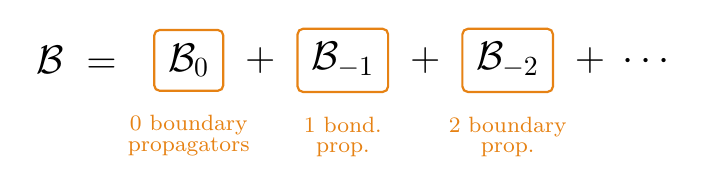
\begin{tikzpicture}[baseline=(Beq.base)]
\node[anchor=west] (Beq) at (0,0) {\Large $\mathcal{B} \;=\;$};
\node[draw=orange1, thick, rounded corners=2pt, inner sep=5pt, anchor=west] (B0) at (1.6,0) {\Large $\mathcal{B}_0$};
\node[anchor=west] (p1) at (B0.east) {\Large $\;+\;$};
\node[draw=orange1, thick, rounded corners=2pt, inner sep=5pt, anchor=west] (Bm1) at (p1.east) {\Large $\mathcal{B}_{-1}$};
\node[anchor=west] (p2) at (Bm1.east) {\Large $\;+\;$};
\node[draw=orange1, thick, rounded corners=2pt, inner sep=5pt, anchor=west] (Bm2) at (p2.east) {\Large $\mathcal{B}_{-2}$};
\node[anchor=west] at (Bm2.east) {\Large $\;+\;\cdots$};
\node[orange1, font=\footnotesize, below=5pt of B0, align=center] {$0$ boundary\\[-2pt] propagators};
\node[orange1, font=\footnotesize, below=5pt of Bm1, align=center] {$1$ bond.\\[-2pt] prop.};
\node[orange1, font=\footnotesize, below=5pt of Bm2, align=center] {$2$ boundary\\[-2pt] prop.};
\end{tikzpicture}

\vspace{0.5cm}

% ============================================================
% FEYNMAN TREE DIAGRAMS n=5
% ============================================================
\begin{center}
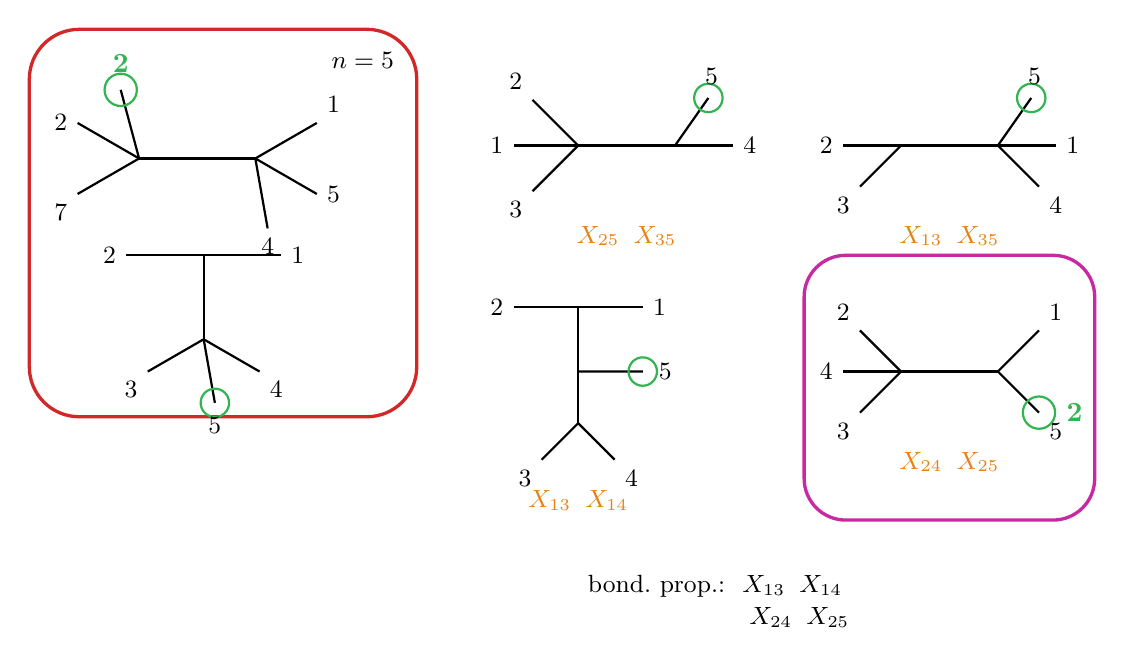
\begin{tikzpicture}[scale=0.82, every node/.style={font=\small}]

% RED OVAL
\draw[red1, very thick, rounded corners=18pt] (-3.0,-3.2) rectangle (3.0, 2.8);
\node[anchor=north east] at (2.8, 2.6) {$n=5$};

% Tree A (top in red oval)
\coordinate (LA) at (-1.3, 0.8);
\coordinate (RA) at (0.5, 0.8);
\draw[thick] (LA)--(RA);
\draw[thick] (LA) -- ++(150:1.1) node[left]{2};
\draw[thick] (LA) -- ++(210:1.1) node[below left]{7};
\coordinate (g2a) at ($(LA)+(105:1.1)$);
\draw[thick] (LA) -- (g2a);
\draw[green1, thick] (g2a) circle(0.25);
\node[green1, font=\bfseries] at ($(g2a)+(0,0.4)$) {2};
\draw[thick] (RA) -- ++(30:1.1) node[above right]{1};
\draw[thick] (RA) -- ++(330:1.1) node[right]{5};
\draw[thick] (RA) -- ++(280:1.1) node[below]{4};

% Tree B (bottom in red oval)
\coordinate (TB) at (-0.3, -0.7);
\coordinate (BB) at (-0.3, -2.0);
\draw[thick] (TB)--(BB);
\draw[thick] (TB) -- ++(0:1.2) node[right]{1};
\draw[thick] (TB) -- ++(180:1.2) node[left]{2};
\draw[thick] (BB) -- ++(210:1.0) node[below left]{3};
\draw[thick] (BB) -- ++(330:1.0) node[below right]{4};
\coordinate (g5b) at ($(BB)+(280:1.0)$);
\draw[thick] (BB) -- (g5b);
\draw[green1, thick] (g5b) circle(0.22);
\node at ($(g5b)+(0,-0.35)$) {5};

% Tree C: X_{25}, X_{35}
\coordinate (LC) at (5.5, 1.0);
\coordinate (RC) at (7.0, 1.0);
\draw[thick] (LC)--(RC);
\draw[thick] (LC) -- ++(135:1.0) node[above left]{2};
\draw[thick] (LC) -- ++(180:1.0) node[left]{1};
\draw[thick] (LC) -- ++(225:1.0) node[below left]{3};
\draw[thick] (RC) -- ++(0:0.9) node[right]{4};
\coordinate (g5c) at ($(RC)+(55:0.9)$);
\draw[thick] (RC) -- (g5c);
\draw[green1, thick] (g5c) circle(0.22);
\node at ($(g5c)+(0.05,0.33)$) {5};
\node[orange1] at (6.25, -0.4) {$X_{25}\;\;X_{35}$};

% Tree D: X_{13}, X_{35}
\coordinate (LD) at (10.5, 1.0);
\coordinate (RD) at (12.0, 1.0);
\draw[thick] (LD)--(RD);
\draw[thick] (LD) -- ++(180:0.9) node[left]{2};
\draw[thick] (LD) -- ++(225:0.9) node[below left]{3};
\draw[thick] (RD) -- ++(0:0.9) node[right]{1};
\draw[thick] (RD) -- ++(315:0.9) node[below right]{4};
\coordinate (g5d) at ($(RD)+(55:0.9)$);
\draw[thick] (RD) -- (g5d);
\draw[green1, thick] (g5d) circle(0.22);
\node at ($(g5d)+(0.05,0.33)$) {5};
\node[orange1] at (11.25, -0.4) {$X_{13}\;\;X_{35}$};

% Tree E: X_{13}, X_{14}
\coordinate (TE) at (5.5, -1.5);
\coordinate (ME) at (5.5, -2.5);
\coordinate (BE) at (5.5, -3.3);
\draw[thick] (TE)--(ME)--(BE);
\draw[thick] (TE) -- ++(0:1.0) node[right]{1};
\draw[thick] (TE) -- ++(180:1.0) node[left]{2};
\coordinate (g5e) at ($(ME)+(0:1.0)$);
\draw[thick] (ME) -- (g5e);
\draw[green1, thick] (g5e) circle(0.22);
\node at ($(g5e)+(0.35,0)$) {5};
\draw[thick] (BE) -- ++(225:0.8) node[below left]{3};
\draw[thick] (BE) -- ++(315:0.8) node[below right]{4};
\node[orange1] at (5.5, -4.5) {$X_{13}\;\;X_{14}$};

% Tree F: X_{24}, X_{25} in MAGENTA oval
\draw[magenta1, very thick, rounded corners=15pt] (9.0,-4.8) rectangle (13.5,-0.7);
\coordinate (LF) at (10.5, -2.5);
\coordinate (RF) at (12.0, -2.5);
\draw[thick] (LF)--(RF);
\draw[thick] (LF) -- ++(135:0.9) node[above left]{2};
\draw[thick] (LF) -- ++(225:0.9) node[below left]{3};
\draw[thick] (LF) -- ++(180:0.9) node[left]{4};
\draw[thick] (RF) -- ++(45:0.9) node[above right]{1};
\draw[thick] (RF) -- ++(315:0.9) node[below right]{5};
\coordinate (g2f) at ($(RF)+(315:0.9)$);
\draw[green1, thick] (g2f) circle(0.25);
\node[green1, font=\bfseries] at ($(g2f)+(0.55,0)$) {2};
\node[orange1] at (11.25, -3.9) {$X_{24}\;\;X_{25}$};

% Bottom summary
\node[anchor=north west] at (5.5, -5.5) {bond.\ prop.:\ \ $X_{13}\;\;X_{14}$};
\node[anchor=north west] at (8.0, -6.0) {$X_{24}\;\;X_{25}$};

\end{tikzpicture}
\end{center}

\end{document}
